\subsection*{How to: W-LAN}

Du bist nun stolzes Mitglied der Goethe-Universität Frankfurt oder schlichtweg begeisterter Interessent für unseren
Fachbereich „Informatik“? Jetzt stellt sich dir nach einer Stunde frustriertem Haareraufen die Frage: „Haben die Freaks
hier kein Internet!?“

Doch klar, aber wir wären doch keine Fachidioten, wenn der Zugang jedem benutzerfreundlich
zugeschoben würde. Deshalb haben wir es uns zur Aufgabe gemacht, den Umstand der Router-Suche, das Feilschen um
notwendige Dateien \& die Durchführung einer Serverwartung unangekündigt genau dann zu starten, wenn du es am wenigsten
erwartest; oder zumindest ließen sich so einige unglaubliche Phänomene ansatzweise begründen.

\begin{center}
	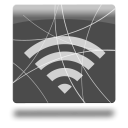
\includegraphics{bitmaps/network-wlan-icon}
\end{center}
\vspace{-5mm}

%%%%%%%%%%%%%%%%%%%%
\subsection*{Minimale Anforderungen}

Ohne dich gleich überfordern zu wollen, musst du dir darüber im Klaren sein, dass du ohne einen Laptop, oder ein „Mobile
Device“ nicht weit kommst. Sollte beides nicht zur Hand sein, ließ erst einmal beim Punkt „W-LAN Versorgung“ weiter.
Falls du die Zeile noch nicht verlassen haben solltest: Um dich mit einem unserer Router zu verbinden, benötigst du
einen HRZ-Account.

\begin{fancyblock}{HRZ?}
	Das Hochschulrechenzentrum stellt euch verschiedene Services zur Verfügung.\\
	Unter anderem den Internetzugang! Mit deiner Erstimmatrikulation hast du deine\\
	HRZ-Login-Daten erhalten, die dir als Identifikationsschlüssel dienen.
\end{fancyblock}

Auf dem Campus müsste dein Rechner verschiedene Netzwerke finden, u.a. FLUGHAFEN, eduroam und FREIFLUG. Was sich auf den
ersten Blick nicht erkennen lässt; hierbei handelt es sich um das gesuchte Angebot an dich eine W-LAN Verbindung
aufzubauen.

Diskutieren wir nicht über die Namen und treffen eine beliebige Wahl. In der unteren, rechten Ecke deines
Bildschirms erscheint nun ein kleines Fenster, in dessen Spalten du dein HRZ-Login und -passwort eintippst (bei FREIFLUG
erfolgt die Authentifizierung über den Browser\footnote{Das Formular erscheint beim Aufruf der ersten Webseite.}).

Das funktioniert sowohl für deinen Laptop, als auch für dein Handy, IPad, etc.

%%%%%%%%%%%%%%%%%%%%
%\subsection*{Hey, ich bin aber kein Student an dieser Uni!}
%
%Ausnahmsweise darfst du trotzdem sitzen bleiben.\\
%Ließ einfach die Erläuterungen zum Vorsemesterkurs.
%
%%%%%%%%%%%%%%%%%%%%
\subsection*{RBI}

Um die Unirechner zu verwenden, die sich in den Fischerräumen finden lassen, benötigst du wiederum andere Login-Daten,
diese werden dir von der RBI zur Verfügung gestellt.

\begin{fancyblock}{RBI?}

Die Rechnerbetriebsgruppe Informatik besteht aus einer Hand voll Linux-Fanatikern, die ihren Sitz
im Keller des Institutsgebäudes beziehen. Solltest du einmal Probleme mit der Internetverbindung haben, folge einfach
der Treppe nach unten ins Dunkel...
\end{fancyblock}

Wenn du am Vorsemesterkurs Informatik teilgenommen hast, wurden dir zu Beginn die entsprechenden Zugangsdaten
ausgeteilt, mit denen du auf die RBI-Rechner zugreifen kannst. Ändere bitte bei der ersten Anmeldung dein Passwort \&
denk nicht einmal darüber nach „Gandalf“ zu verwenden; hier ist ein wenig Kreativität gefordert! Merke: Unsichere Passworte können zur Accountsperrung führen! 

Deinen RBI-Account benötigst du nicht nur für die Unirechner, sondern auch um das RBI-Netzwerk nutzen zu können und
später für das Praktikum. Im Fall, dass du den Vorsemesterkurs verschwitzt hast, begebe dich einfach in den Keller des
Institutsgebäudes und bitte die Mitarbeiter der RBI dir ein Konto zu eröffnen.

\begin{fancyblock}{WARNUNG!}

Bevor dir deine Daten ausgehändigt werden, wirst du dazu angehalten eine entsprechende
Zustimmungserklärung zu unterzeichnen, in der du dich dazu verpflichtest, deine Daten geheim zu halten. Sollte mit
deinem Account Unfug getrieben werden, kommen wir auf dich zurück!
\end{fancyblock}

\begin{fancyblock}{RBI-Netzwerk?}

Parallel zum HRZ bietet die RBI ebenfalls  den WLAN-Zugriff über ein eigenes Netzwerk an.
Sollte irgendwann ein HRZ-Access Point durch 20 andere Studierende überlastet sein, bleibt dir noch
der Ausweg zum OpenVPN Netzwerk der RBI zu wechseln.
\end{fancyblock}

%%%%%%%%%%%%%%%%%%%%
\subsection*{OpenVPN}

Dein RBI-Account ist nicht nur für die Fischerräume notwendig, sondern ermöglicht dir auch innerhalb des
Institutsgebäudes (zzgl. Matheturm) den Zugang zu einem weiteren Netzwerk.

Hier kommst du mit deinen Daten allein leider nicht mehr weiter:
\begin{enumerate}
	\item Wähle das OpenVPN Netzwerk aus, öffne deinen Browser und rufe eine beliebige Seite auf.

	Bevor du die Verbindung im ganzen Ausmaß nutzen kannst, bist du gezwungen dir einige Dateien für dein Betriebssystem herunterzuladen.
	\item Ist dir der Prozess geglückt, starte bitte das beinhaltete OpenVPN GUI Programm mit Administratorrechten (wichtig!).
	\item Vollziehe einen Rechtsklick auf das zugehörige Icon in deiner Taskleiste und wähle „connect“, im Anschluss wirst du dazu aufgefordert
	deine RBI-Daten einzutippen.

	Versuche es erst gar nicht mit den HRZ-Daten. Der RBI-Login beinhaltet deinen Namen (nicht	zu verwechseln)!
	\item  Bei Bedarf bitte nicht verzweifeln, bediene dich des „Reconnect's“!
\end{enumerate}

\begin{fancyblock}{Der OpenVPN-Bonus}

In einigen Stöcken des Matheturms, wo der Signal von HRZ-Netzwerken sehr schwach ist,
lässt sich mit OpenVPN eine Internetverbindung herstellen. Ihr müsst hierzu die IP-Adresse in der Konfigurationsdatei
austauschen. Eine Anleitung findet sich in eurem Browser, wenn ihr versucht auf das Netzwerk zuzugreifen und eine
beliebige Webseite aufzurufen..
\end{fancyblock}

%%%%%%%%%%%%%%%%%%%%
\subsection*{W-LAN Versorgung \& Fehlerbehebung}

\begin{itemize}
	\item \textbf{Ich besitze keinen eigenen Laptop!}

	Nutze bitte einen der lokalen Unirechner in den Fischerräumen.
	
	\item \textbf{Mein Rechner findet einfach kein Netzwerk!}

	\begin{tabular}{p{0.2\linewidth}p{0.77\linewidth}}
\rule{0pt}{2ex} 
	Fischerräume: & Nutze die lokalen Rechner, dafür sind sie da!\\
\rule{0pt}{4ex} 
	Mathe-Turm: & Hier sind nicht alle Stöcke mit dem WLAN versorgt.

	Melde dich mit den Beschwerde, bitte, bei der Mathe-Fachschaft: fachschaft@math.uni-frankfurt.de\\
\rule{0pt}{4ex} 
	Lernzentrum, &  Finde oben ein weißes Access Point.  Sollte darauf ein grünes oder\\
\rule{0pt}{0ex} 
	Student Lounge, & ein blaues LED leuchten, liegt das an deinen WLAN-Einstellungen.\\
\rule{0pt}{0ex} 
	SR11 und SR307: & Sollte das LED rot leuchten, teile das dem HRZ-Team mit:

	wlan-fragen@rz.uni-frankfurt.de\\
\rule{0pt}{4ex} 
	Magnus, SR9: & Melde dich mit deiner Beschwerde bitte bei der RBI.\\
\rule{0pt}{4ex} 
	Weitere Infos: & \url{www.rz.uni-frankfurt.de/campusnetz/wlan/flugplatz/cb.html}
	\end{tabular}
\end{itemize}

\begin{fancyblock}{OpenVPN funktioniert plötzlich nicht mehr!}
Entweder du hast die falsche IP-Adresse in deiner Konfigurationsdatei auskommentiert,
oder bei der letzten Reinigung deines Rechners ging eine wichtige Datei verloren.
In diesem Fall empfiehlt es sich das Paket für dein Betriebssystem erneut downzuloaden.
\end{fancyblock}

\begin{flushright}Sabrina \& Pavel \end{flushright}

%\vspace{3mm}
%\begin{center}
%	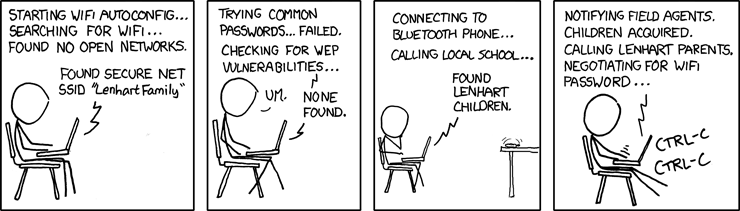
\includegraphics[scale=0.42]{bitmaps/zealous_autoconfig}
%\end{center}
